\section{Conception UML}
\subsection{Liste des objets}
\begin{itemize}
\item Gare : code gare, composé d'un nom, d'une addresse, d'une ville, d'un nombre de quai
\item Rame : composé d'un numéro,d'une modèle, d'un nombre de place 1er, d'un nombre de place 2ème
\item Conducteur : composé d'un Nom, prénom, No secu, No d'identifiant

\item Trajet : composé d'un numero, d'une gare de départ, d'une gare d'arrivée, d'un train, d'un conducteur, date de depart, d'une duréé de trajets

\end{itemize}

\subsection{Relation}
\begin{itemize}
\item Un trajet est composé d'une Rame conduit par un conducteur, depuis une gare de depart à l'heure de départ vers une gare d'arrivé pendant une durée de trajet
\end{itemize}
\subsection{Graph uml}
\begin{figure}[h]
   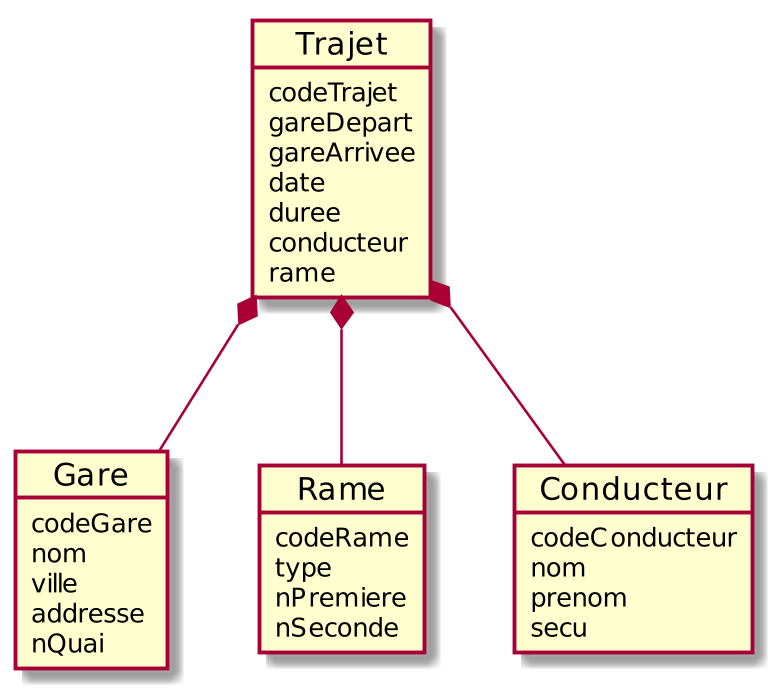
\includegraphics[width=1.0\textwidth]{uml.png}
\end{figure}
%%% Local Variables:
%%% mode: latex
%%% TeX-master: t
%%% End:
